\chapter{Introducción a Árboles}
En este tema vamos a ver todo sobre los árboles que se usan en programación.

Encontraremos varios tipos de árboles (binarios, generales, ABB, APOs, entre otros), que nos facilitarán el trabajo a la hora de resolver algunos problemas.

Para poder entender todos los conceptos que vamos a dar sobre los árboles, primero debemos de entender qué es un árbol.

Los árboles ofrecen dos ventajas frente a las estructura de datos lineales (listas, vectores, colas, etc..):
\begin{itemize}
  \item Permiten representar \textbf{jerarquías}.
  \item En algunos casos podemos realizar búsquedas de \textbf{orden logarítmicas}: \(O(log\ n)\).
\end{itemize}
\section{Definición de árbol}

Un árbol en el ámbito de la programación es un conjunto de elementos de un tipo determinado, donde cada elemento se almacena en un \textbf{nodo}.\\
En los árboles vamos a encontrar una \textit{relación de paternidad} (padre - hijo) entre los diferentes nodos que conforman el árbol, como veremos en la \textit{Figura 1.1}.

\begin{figure}[h]
  \begin{center}
    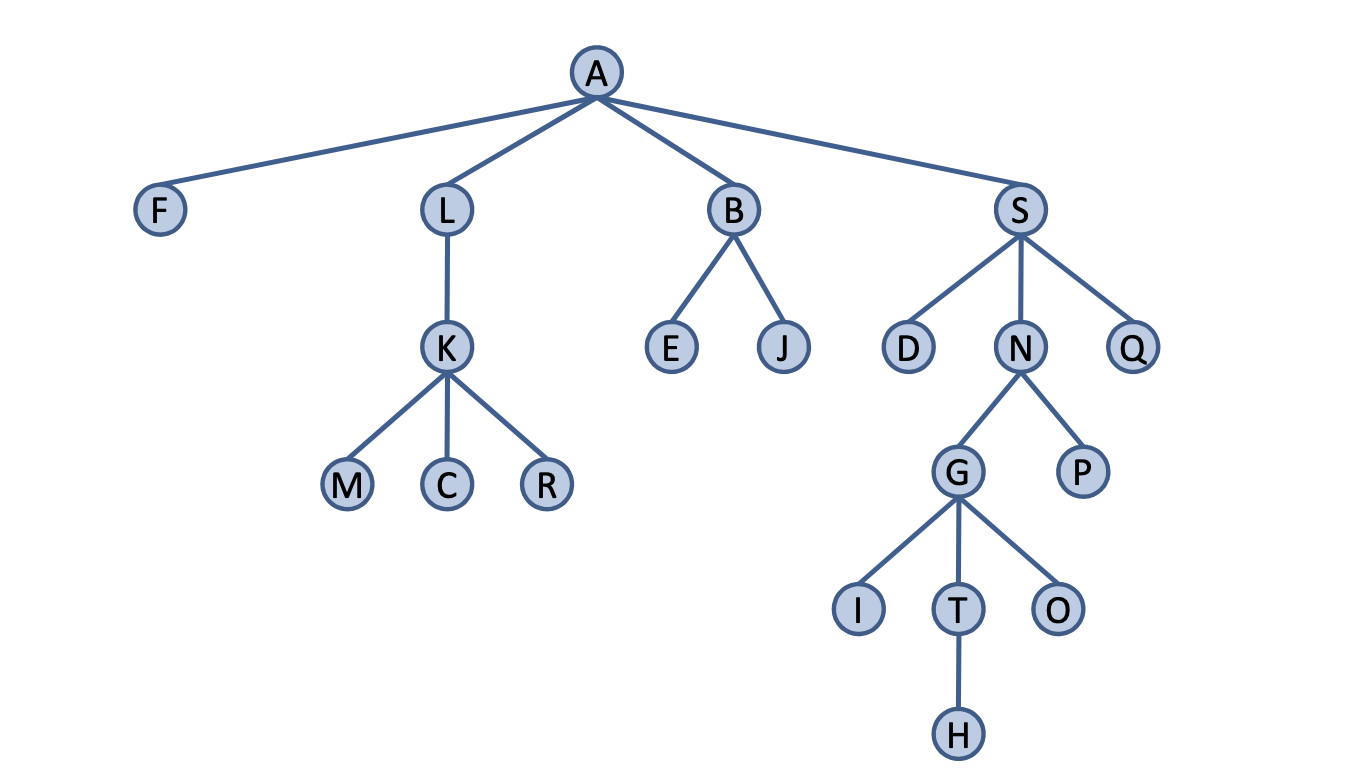
\includegraphics[width=\textwidth]{assets/IntroArboles1.png}
  \end{center}
  \caption{Ejemplo de árbol}
  Cada letra sería un nodo diferente.\\
  Por ejemplo: el nodo A es padre de los nodos F, L, B y S.
\end{figure}

\newpage
\underbar{Una definición más formal sería:}

Si \texttt{n} es un \textbf{nodo} y \texttt{$A_1$, $A_2$, ..., $A_k$} son árboles con raíces \texttt{$n_1$, $n_2$, ..., $n_k$} y además se define una relación de paternidad (siendo hijos de \texttt{n} y hermanos entre sí), tenemos como resultado un árbol (\textit{Figura 1.2:Definición de árbol}).

Si solamente tenemos un único nodo, en nuestro caso \texttt{n}, diremos que tenemos un \textbf{árbol vacío}.

\begin{figure}[h]
  \begin{center}
    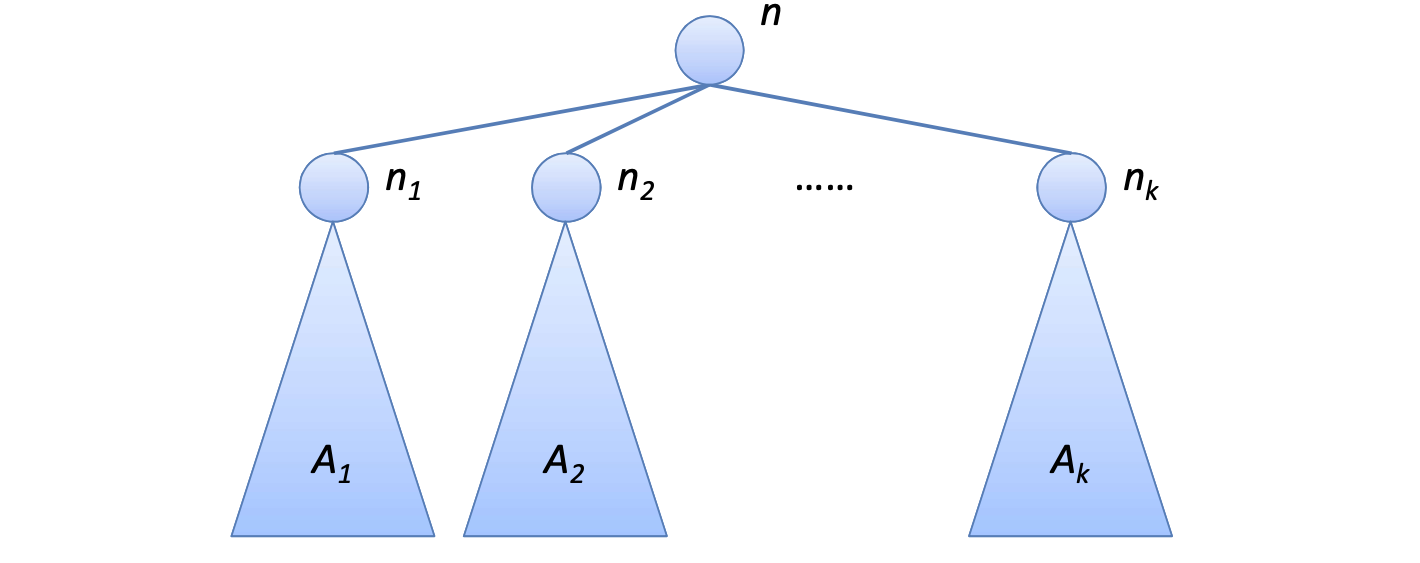
\includegraphics[width=\textwidth]{assets/IntroArboles2.png}
  \end{center}
  \caption{Definición de árbol}
  Vemos que \texttt{$A_1$, $A_2$, ..., $A_k$} son subárboles cuyas raíces son los nodos {$n_1$, $n_2$, ..., $n_k$} que a su vez son hijos del nodo \texttt{n} (raíz del árbol).
\end{figure}

\section{Definiciones}
Vamos a ver varias definiciones sobre algunos conceptos de los árboles como (grado, camino, longitud, etc).

\underbar{\large\textbf{Grado:}} El grado es el número de nodos hijos de un nodo en concreto. El grado del árbol es el máximo de los grados de los nodos que lo componen.
\begin{figure}[h]
  \begin{center}
    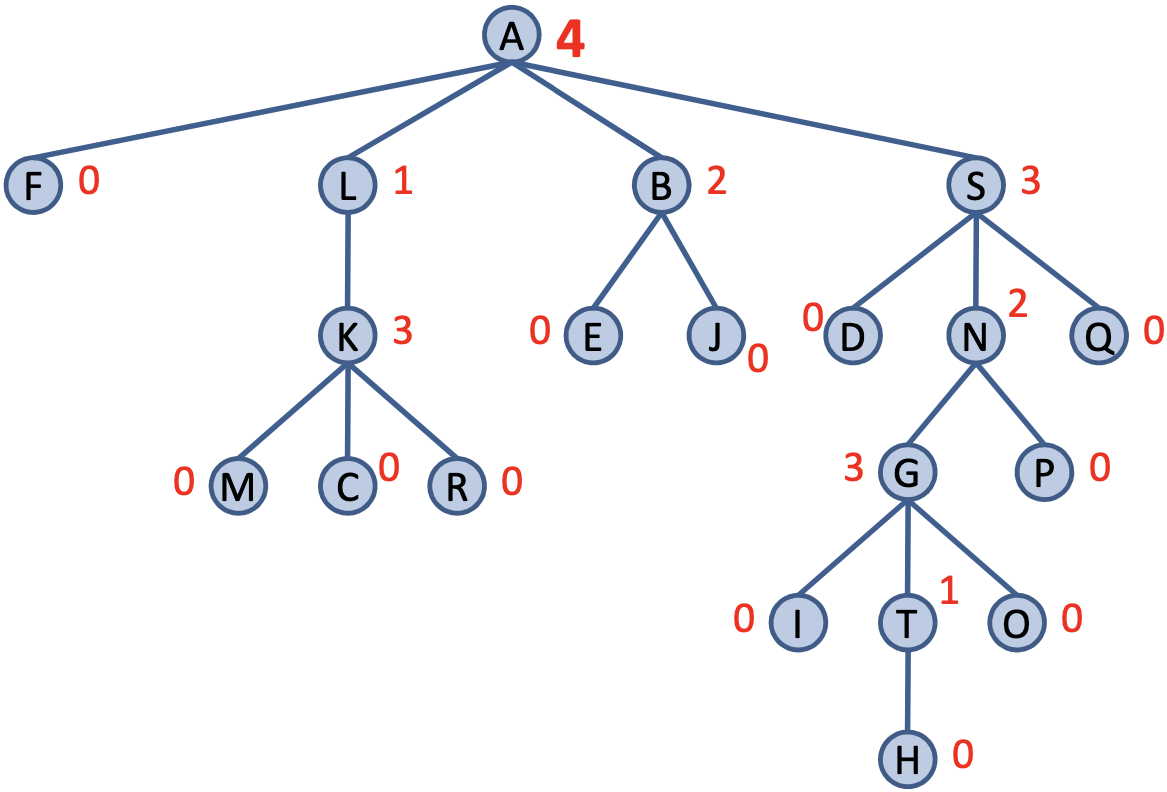
\includegraphics[width=0.6\textwidth]{assets/IntroArboles3.png}
  \end{center}
  \caption{Grado de un árbol}
  \textit{Nota}: El grado de un árbol no tiene porque ser siempre igual al grado del nodo raíz.
\end{figure}

\underbar{\large\textbf{Camino y Longitud:}} El camino es una suceción de nodos del árbol \texttt{$n_1$, $n_2$, ..., $n_k$} donde  \texttt{$n_1$} es el padre de  \texttt{$n_i$+1}. El camino no tiene porque empezar en la raíz del árbol, es decir, se puede realizar un camino desde cualquier nodo.

La longitud de un árbol es el número de nodos - 1.

\begin{figure}[h]
  \begin{center}
    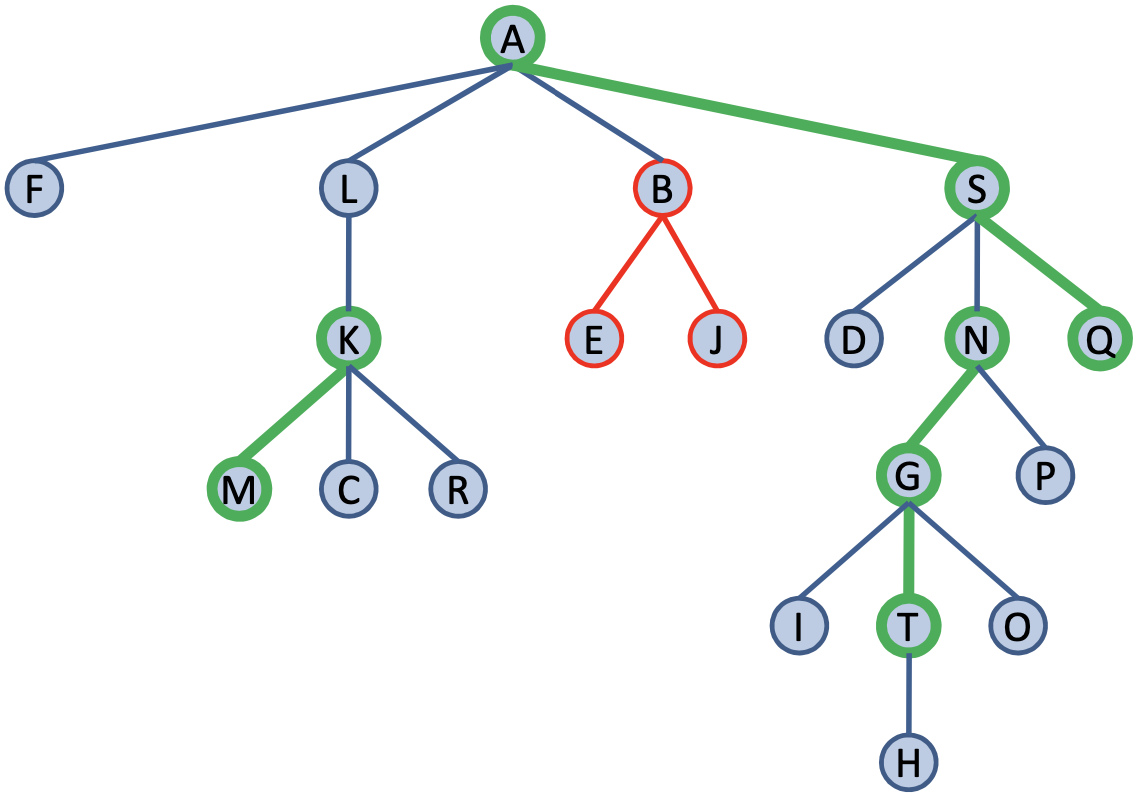
\includegraphics[width=0.6\textwidth]{assets/IntroArboles4.png}
  \end{center}
  \caption{Camino y Longitud de un árbol}
  En verde encontramos tres ejemplos de caminos diferentes.
\end{figure}

\underbar{\large\textbf{Ancestros y Descendientes:}} Si existe un camino entre dos nodos \textit{a} y \textit{b} cualesquiera, el nodo \textit{a} será \textbf{antecesor/ancestro} del nodo \textit{b} y el nodo \textit{b} será \textbf{descendiente} del nodo \textit{a}.

Si ese ancestro o descendiente son su padre o hijo(s)(respectivamente), se denominarán \textbf{ancestro propio} ó \textbf{descendiente propios}.

\begin{figure}[h]
  \begin{center}
    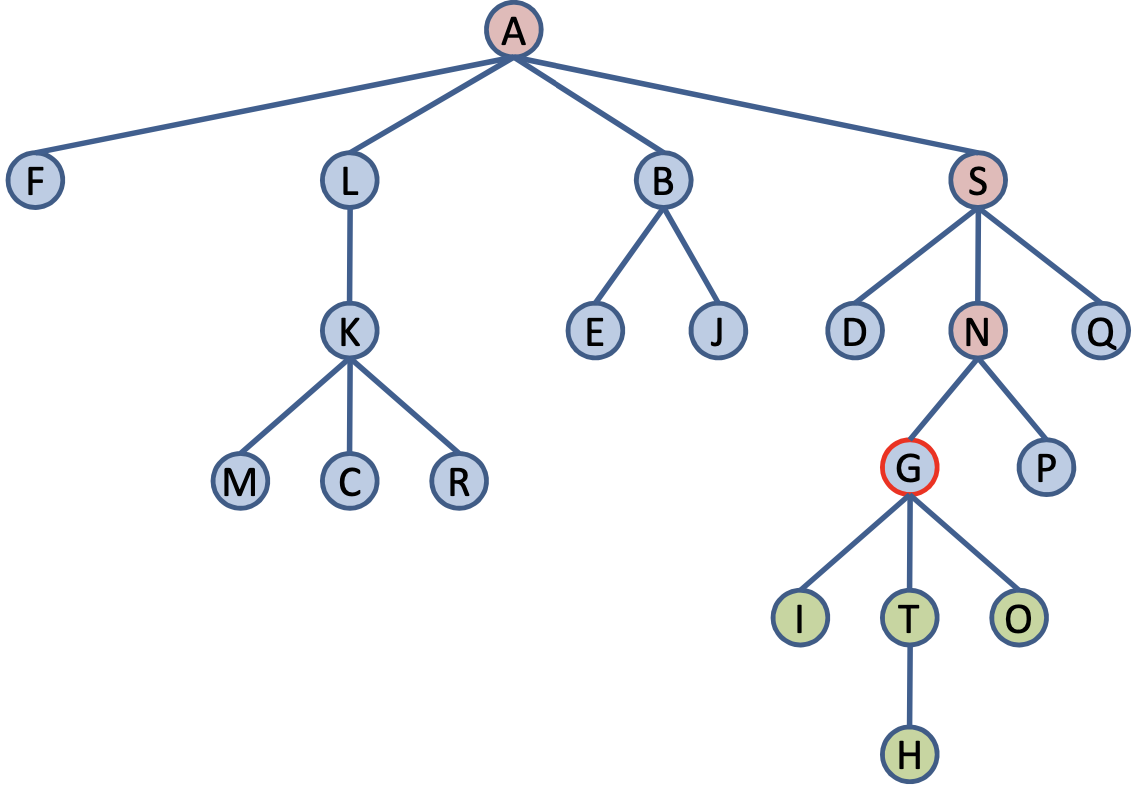
\includegraphics[width=0.6\textwidth]{assets/IntroArboles5.png}
  \end{center}
  \caption{Ancestros y Descendientes de un nodo}
  Vemos que el nodo A tiene como descendientes propios los nodos (F, L, B, S) y como descendientes los hijos de estos anteriores.
\end{figure}
\newpage
\section{Componentes de un árbol}

Los árboles se componen de nodos raiz, hojas, subárboles, ramas, etcétera.

\underbar{\large\textbf{Raíz:}} Es el único nodo del árbol que no tiene ancestro.

\underbar{\large\textbf{Hoja:}} Es aquel nodo que no tiene ningún descendiente propio y por ende no tiene descendientes. \(\textbf{Hoja}\neq\textbf{árbol nulo}\).

\underbar{\large\textbf{Subárbol:}} Conjunto formado por un nodo cualquiera y sus descendientes.

\underbar{\large\textbf{Rama:}} Es el camino que termina en un nodo que es hoja.

\begin{figure}[h]
  \begin{center}
    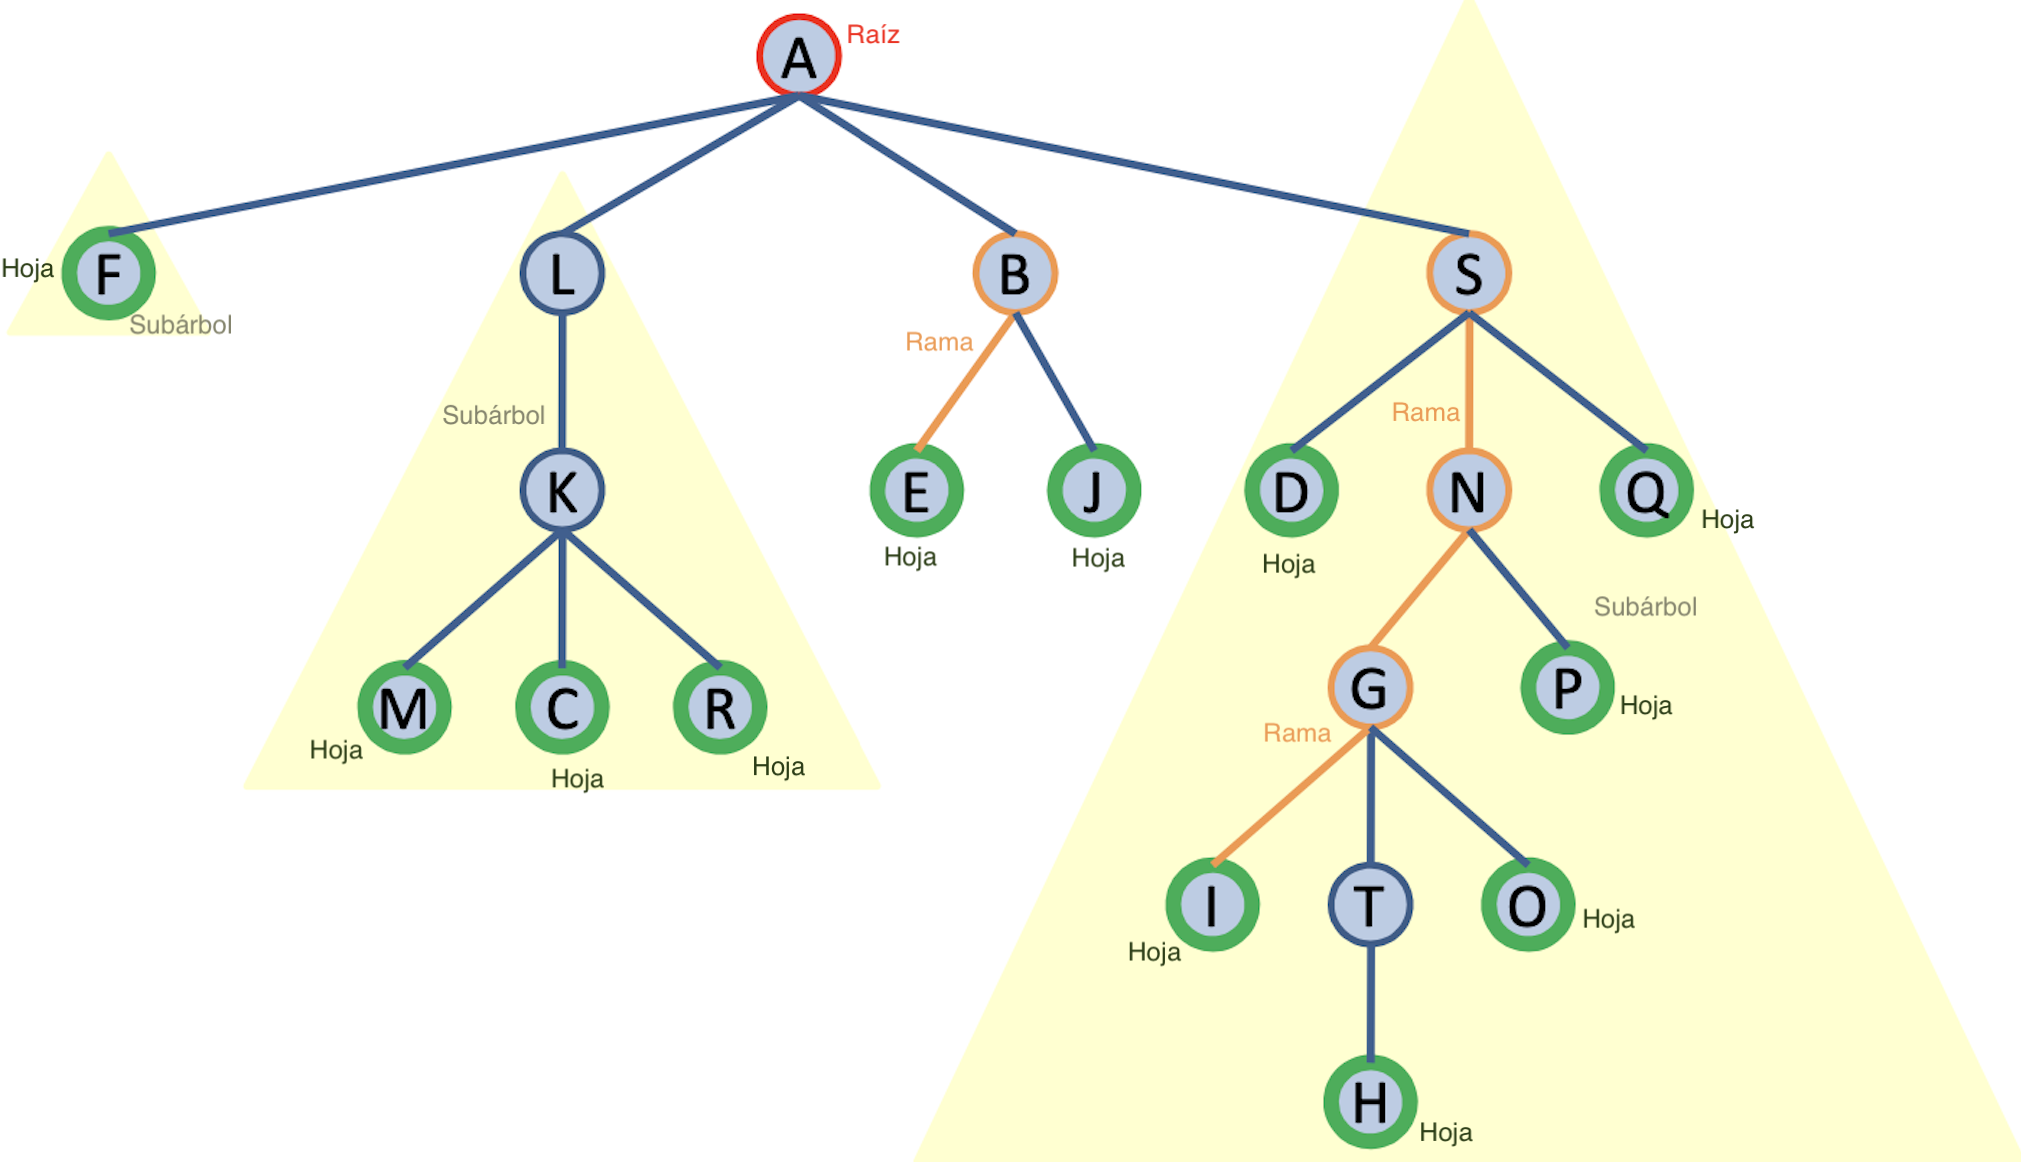
\includegraphics[width=\textwidth]{assets/IntroArboles6.png}
  \end{center}
  \caption{Componentes de un árbol}
  En el nodo F, tenemos dos puntos de vista:
  \begin{itemize}
    \item Respecto al súbarbol, es raíz sin descendientes propios (hoja).
    \item Respecto al árbol, es una hoja.
  \end{itemize}
\end{figure}
\newpage
\underbar{\large\textbf{Altura y Profundidad:}}
\begin{itemize}
  \item La Altura es la longitud de la rama más larga, la altura del árbol se corresponde con la altura del nodo raíz.
  \item La Profundidad es la longitud desde el único camino desde la raíz hasta ese nodo. También se denomina \textit{nivel de nodo}.
\end{itemize}

\begin{figure}[h]
  \begin{center}
    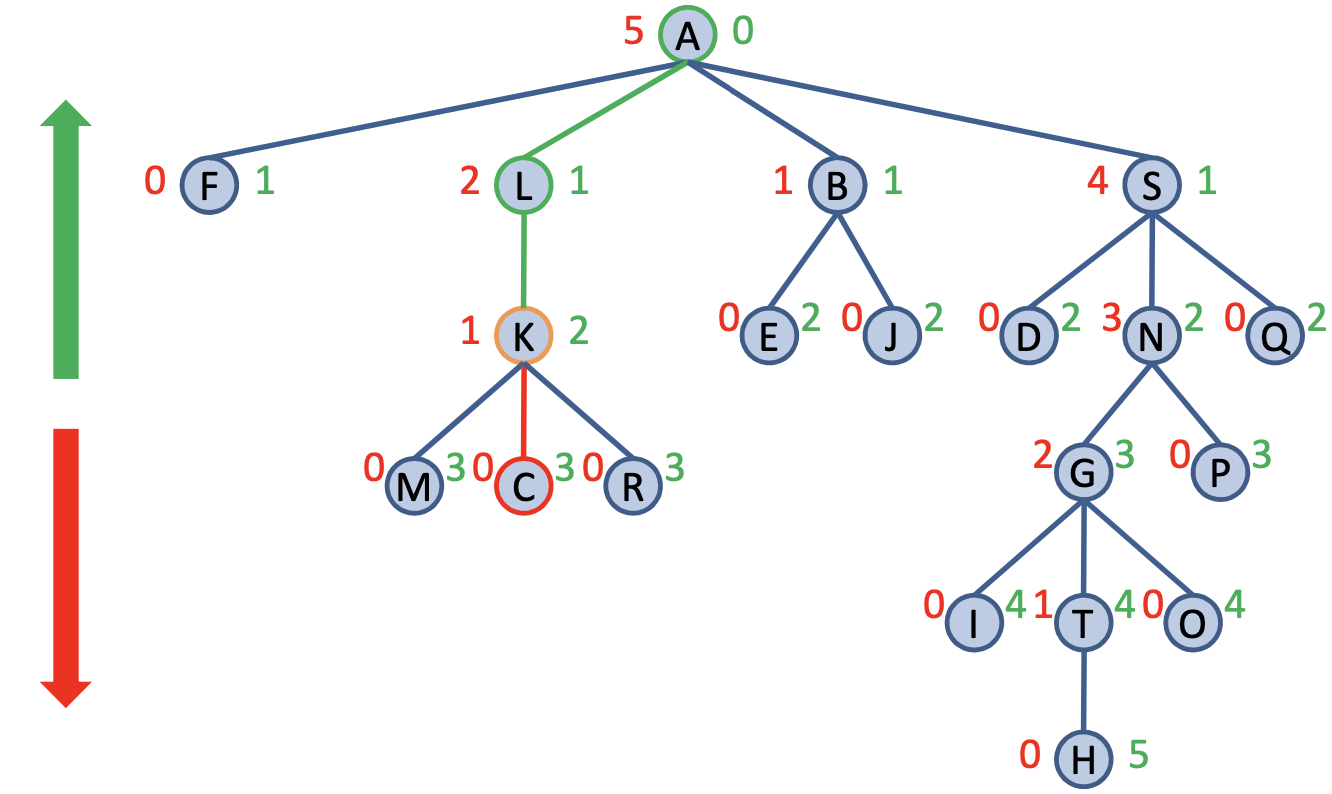
\includegraphics[width=0.5\textwidth]{assets/IntroArboles7.png}
  \end{center}
  \caption{Ejemplo de altura y profundidad}
  En rojo vemos la altura y en verde la profundidad.
\end{figure}